\chapter{Marco de Referencia}

 Desde finales del siglo pasado, los avances tecnológicos en la miniaturización de la electrónica y los componentes mecánicos han allanado el camino para la creación y desarrollo de objetos voladores de pequeñas dimensiones, tales como aviones y helicópteros, los cuales están adquiriendo cada vez más habilidades para realizar vuelos de forma autónoma. Estos dispositivos son popularmente conocidos como drones, un término derivado del inglés \say{abejorros}, y se consideran máquinas voladoras autónomas o semi-autónomas capaces de llevar a cabo misiones de vuelo. En el ámbito internacional, se les conoce como UAVs del ingles \say{Unmanned Aerial Vehicles}, y representan una tecnología compleja cuyo control presenta desafíos, dado que sus características aerodinámicas son similares a las de las aeronaves convencionales \cite{eisenbeiss2004mini}.

El estudio de estos dispositivos despierta un gran interés debido a su versatilidad y capacidad de maniobra, lo que les permite llevar a cabo una amplia gama de tareas en diversas aplicaciones, tales como el uso civil, militar y aeroespacial \cite{nawaz2019applications, shakhatreh2019unmanned, xiaoning2020analysis}. En la figura \ref{fig1_aplicacion_UAV}, se presenta una clasificación detallada de las aplicaciones más importantes de los UAVs.

\begin{figure}[H]
    \centering
    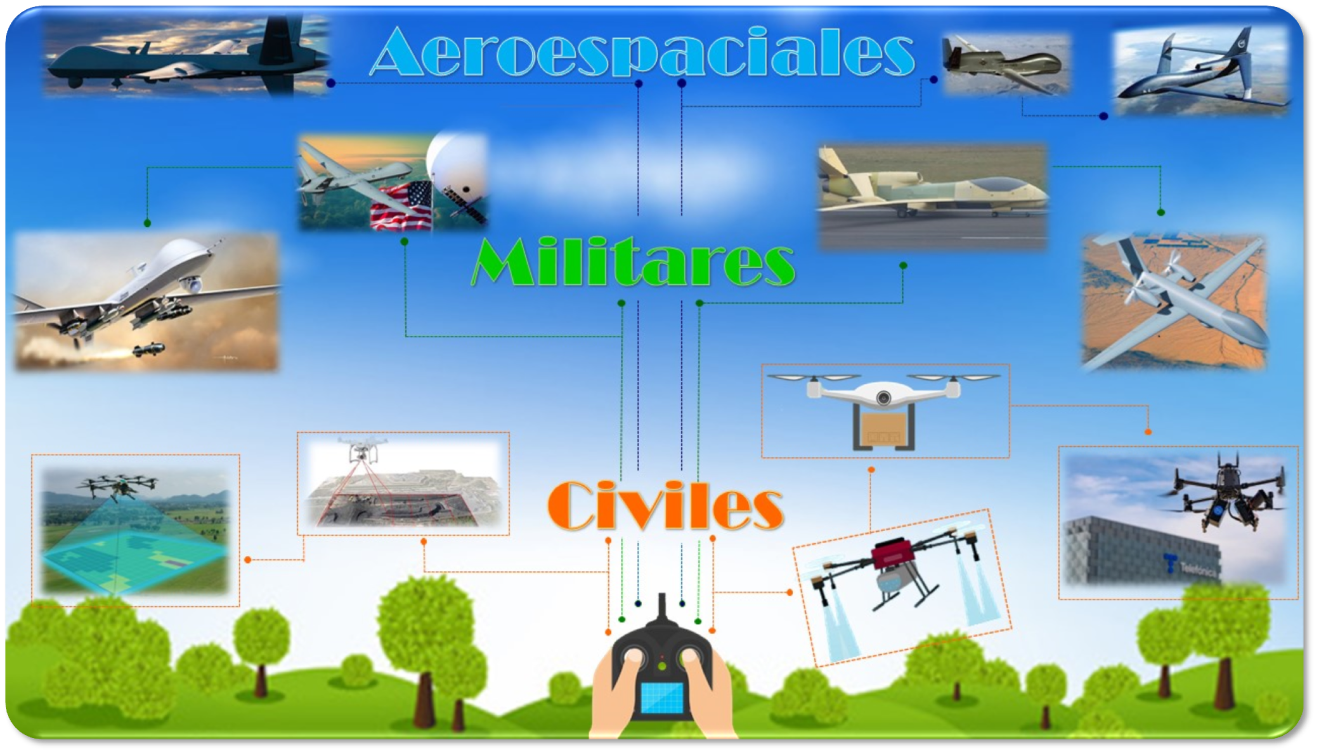
\includegraphics[width=16cm, height=7.5cm]{imagenes/Aplicaciones_UAV.png}
    \caption{Áreas de aplicación UAVS.}
    \label{fig1_aplicacion_UAV}
\end{figure}

\section{Antecedentes.}

Los drones han atraído la atención de la comunidad investigadora que trabaja tanto en el campo militar como en el civil, con una gran cantidad de usos que han sido propuestos por los grupos de investigación, debido a sus características como capacidad y configuraciones, donde el helicóptero de cuatro rotores tiene el mayor número de citas en la literatura de control y ha sido ampliamente investigado para pruebas tanto en interiores como en exteriores . 

\section{Objetivo General}

Desarrollar un sistema web de gestión y control de inventarios multi-tenant, utilizando el framework Laravel, una arquitectura Modelo-Vista-Controlador (MVC) extendida con una capa de servicios y una base de datos relacional, mejorando la eficiencia, organización y precisión de los procesos de administración de inventarios de distintos tipos de establecimientos, permitiendo la personalización de módulos, el control de existencias y la gestión independiente y segura de la información de cada organización.

\section{Objetivos Específicos}
\begin{enumerate}
    \item Identificar las problemáticas y necesidades relacionadas con la gestión de inventarios en establecimientos de abarrotes, farmacias, bibliotecas, papelerías y equipos electrónicos, mediante la aplicación de cuestionarios, entrevistas y el análisis de sus procesos administrativos, para determinar los requerimientos funcionales y no funcionales del sistema.
    \item Estructurar la arquitectura del sistema mediante el patrón Modelo-Vista-Controlador (MVC) extendido con una capa de servicios, estableciendo la organización de componentes, reglas de negocio y mecanismos de comunicación necesarios para su funcionamiento.
    \item Modelar una base de datos relacional normalizada que permita la administración de la información de usuarios, organizaciones, productos, existencias, movimientos, módulos, suscripciones y operaciones, garantizando la integridad de los datos y su separación lógica entre tenants.
    \item Construir un módulo de administración general que permita al superadministrador la gestión de las solicitudes de nuevos tenants, configuración de sus características, administración de planes de suscripción y supervisión del funcionamiento general de la plataforma.
    \item Establecer mecanismos de autenticación, autorización y control de acceso basados en roles y permisos, garantizando que los usuarios únicamente puedan consultar y modificar la información correspondiente a sus responsabilidades y organización.
    \item Programar los módulos generales y específicos para la administración de inventarios, incorporando funcionalidades de registro de productos, control de existencias, movimientos de stock, ventas, bajas, préstamos, devoluciones, lotes, caducidades y mantenimiento de equipos, según las necesidades de cada establecimiento.
    \item Diseñar interfaces web intuitivas y responsivas utilizando Laravel y plantillas Blade, facilitando la interacción de superadministradores, administradores y encargados con las funcionalidades correspondientes a sus roles.
    \item Desplegar el sistema web MULTIVERSE en un entorno de alojamiento mediante la plataforma Hostinger, realizando la configuración de los servicios, la base de datos y los recursos necesarios, con la finalidad de garantizar su correcto funcionamiento, disponibilidad y acceso seguro a través de internet.
\end{enumerate}

\section{Alcance}

\subsection{Arquitectura y Plataforma Multi-Tenant}

\begin{itemize}
    \item \textbf{Aislamiento Multi-Tenant:} La plataforma permitirá gestionar múltiples inventarios de manera totalmente independiente sobre una misma infraestructura física y base de datos compartida, utilizando filtrado de seguridad por clave de tenant (\texttt{tenant\_id}).

    \item \textbf{Patrón de Arquitectura:} Implementación de un patrón MVC extendido mediante una Capa de Servicios dedicada a concentrar las reglas de negocio, validaciones e idempotencia.

    \item \textbf{Módulos Adaptables:} Soporte para los tipos de inventarios predefinidos (Abarrotes, Farmacia, Biblioteca, Papelería y Equipos Electrónicos).
\end{itemize}

\subsection{Gestión de Pagos y Suscripciones de Tenants}

\begin{itemize}
    \item \textbf{Suscripción y Mantenimiento del Servicio:} Integración de un módulo de pagos para que el Administrador del tenant pueda realizar el pago por el uso de la plataforma.

    \item \textbf{Control Automático de Vigencia:} Control y suspensión automática o manual del acceso al inventario y credenciales según la vigencia del pago registrado.
\end{itemize}

\subsection{Gestión de Usuarios y Accesos (RBAC)}

\begin{itemize}
    \item \textbf{Roles Granulares:} Implementación de un control de acceso basado en roles con perfiles como: Superadministrador, Administrador de Inventario, Encargado de Almacén, Encargado de Ventas/Préstamos y Encargado Técnico.

    \item \textbf{Seguridad y Flujo de Invitación:} Registro de solicitudes públicas, generación de credenciales con contraseña temporal obligatoria de primer cambio y hashing seguro para el almacenamiento de contraseñas.
\end{itemize}

\subsection{Funcionalidades Operativas y Módulos}

\begin{itemize}
    \item \textbf{Punto de Venta (POS) e Idempotencia:} Procesamiento de ventas en tiempo real con descuento automático de existencias y mecanismos de idempotencia en backend para evitar duplicidad de transacciones.

    \item \textbf{Mantenimiento y Trazabilidad (Escaneo QR / Barras):} Módulo para captura y consulta de productos mediante lectura de códigos de barras y códigos QR, permitiendo a encargados técnicos registrar servicios de mantenimiento y cambios de estado.

    \item \textbf{Carga Masiva y Exportación:} Soporte para la importación del catálogo inicial a través de archivos de plantilla CSV.

    \item \textbf{Personalización por Tenant:} Capacidad para que el Administrador modifique la identidad visual de su inventario (subida de logotipo, selección de paleta de colores y tema claro/oscuro) y habilite/deshabilite módulos permitidos.

    \item \textbf{Políticas de Soft Delete:} Aplicación de desactivación lógica (\textit{Soft Delete}) en lugar de eliminación física para tenants, productos y usuarios, preservando el historial y la auditabilidad.
\end{itemize}


\section{Limitación}

\subsection{Facturación Electrónica Fiscal}

\begin{itemize}
    \item \textbf{Comprobantes No Fiscales:} No se generarán timbrados ni facturas fiscales oficiales conectadas a organismos tributarios; únicamente se expedirán comprobantes de venta o tickets de carácter informativo interno.
\end{itemize}

\subsection{Restricciones del Multi-Tenant e Inmutabilidad}

\begin{itemize}
    \item \textbf{Inmutabilidad del Tipo de Tenant:} Un administrador no podrá cambiar el tipo de inventario asignado originalmente por el Superadministrador una vez creado el registro.

    \item \textbf{Incompatibilidad Trans-Tenant:} No habrá comunicación, traspaso directo de mercancía ni intercambio de datos entre diferentes tenants o cuentas de inventarios.
\end{itemize}

\subsection{Hardware y Entorno Offline}

\begin{itemize}
    \item \textbf{Dependencia de Conectividad:} El sistema funcionará exclusivamente como una aplicación web en línea; no contará con modo fuera de línea (offline) ni sincronización posterior.

    \item \textbf{Integración de Hardware Limitada:} El escaneo de códigos de barras y códigos QR dependerá del hardware del cliente (lectores USB plug-and-play o la cámara nativa del dispositivo); el sistema no incluirá controladores (drivers) nativos para impresoras térmicas específicas ni periféricos industriales.
\end{itemize}

\subsection{Personalización Estructural de Datos}

\begin{itemize}
    \item \textbf{Esquema de Base de Datos Fijo:} Los campos personalizados por producto se limitarán a atributos predefinidos simples (texto, número, fecha, sí/no), sin posibilidad de alterar la estructura física de las tablas del motor de base de datos en tiempo de ejecución.
\end{itemize}

\section{Problemática}


\section{Justificación}

